\documentclass[11pt]{article}

\usepackage[margin=1in]{geometry}
\usepackage{amsmath,amssymb,amsthm,mathtools}
\usepackage{bm}
\usepackage{graphicx}
\usepackage{booktabs}
\usepackage{tabularx}
\usepackage{enumitem}
\usepackage[dvipsnames]{xcolor}
\usepackage[round,authoryear]{natbib}
\usepackage{microtype}
\usepackage{setspace}
\usepackage[colorlinks=true,linkcolor=MidnightBlue,citecolor=MidnightBlue,urlcolor=MidnightBlue]{hyperref}

\setstretch{1.12}
\setlist{itemsep=2pt,topsep=4pt}

\newtheorem{theorem}{Theorem}
\newtheorem{proposition}{Proposition}
\newtheorem{lemma}{Lemma}
\newtheorem{corollary}{Corollary}
\newtheorem{conjecture}{Conjecture}
\theoremstyle{definition}
\newtheorem{assumption}{Assumption}
\newtheorem{definition}{Definition}
\newtheorem{remark}{Remark}
\newtheorem{observation}{Numerical observation}

\newcommand{\E}{\mathbb{E}}
\newcommand{\Var}{\mathrm{Var}}
\newcommand{\R}{\mathbb{R}}
\newcommand{\sil}{\varnothing}
\newcommand{\sd}{\sigma_d}
\newcommand{\sth}{\sigma_\theta}
\newcommand{\se}{\sigma_\varepsilon}

\title{\textbf{Who Lowers the Bar?}\\[4pt]
\large Expectation Management with a Bayesian Audience}
\author{Preliminary draft --- not for circulation}
\date{September 2026}

\begin{document}
\maketitle

\begin{abstract}
\noindent Before a seminar, a pitch, or a debate, people talk about the circumstances of their upcoming performance: the project is preliminary, the data are poor, the problem is hard. A Bayesian audience cannot be talked into lower expectations on average, and unverifiable claims about circumstances carry no information. Verifiable information about circumstances does matter, because it changes how much of the performance the audience attributes to talent. We study an agent of unknown talent who can disclose evidence about her circumstances before an evaluator observes her performance and decides whether to hire her. The agent discloses exactly when disclosure would raise her assessment at the performance that would be pivotal if she stayed silent. A Bayesian evaluator blames circumstances for disappointments and credits them for surprises. A favorite is pivotal after a disappointment, an underdog after a surprise. As a result, favorites do not lower the bar even when their circumstances are harder than the evaluator would assume, while underdogs raise it. In a Gaussian specification the disclosure threshold is linear in the agent's lead, with slope equal to the ratio of circumstance uncertainty to talent uncertainty. When circumstances affect only how noisy the performance is, favorites announce that it is ``preliminary'' and underdogs that it is ``polished''. Excuses made after the performance do not depend on standing at all.

\medskip
\noindent\textit{Keywords:} expectation management, verifiable disclosure, attribution, career concerns, reference points.\\
\textit{JEL:} D82, D83, D91, M51.
\end{abstract}

\newpage

%======================================================================
\section{Introduction}
%======================================================================

A speaker who opens a seminar with ``this is very preliminary; please don't expect much'' is trying to set the bar against which the talk will be judged. The practice is everywhere. Campaigns lower expectations before debates, firms walk analysts' forecasts down to beatable levels before earnings announcements \citep{Matsumoto2002,RichardsonTeohWysocki2004}, and athletes mention injuries before a race. The folk rule is to underpromise and overdeliver: lower the audience's expectations so that the performance comes as a pleasant surprise.

Against a Bayesian audience the folk rule faces two obstacles. First, expectations are a martingale. Whatever the speaker says, the audience's expected surprise is zero, so no strategy produces pleasant surprises on average (Proposition~\ref{prop:benchmarks}(a)). Second, unverifiable claims about one's circumstances are cheap talk. Every speaker would like the audience to believe that her circumstances are hard, so such claims carry no information (Proposition~\ref{prop:benchmarks}(b)). If lowering expectations works, it cannot work the way the folk rule says.

This paper shows that expectation management does have bite with a Bayesian audience. It works through a different channel, and it is used by different people than the folk rule suggests. The channel is \emph{attribution}. An audience that is learning about a speaker's talent reads her performance against what her circumstances would lead it to expect: the same talk is more impressive if the project is at an early stage. Being judged relative to expectations is therefore not a psychological bias here. It is what Bayesian inference about a person looks like when performance mixes talent with circumstances. Verifiable information about circumstances (the stage of a project, the quality of the data, the strength of the opposition) changes that reading.

We study the simplest environment with this feature. An agent of unknown talent is evaluated on a single performance, which depends on her talent and on her \emph{context}, meaning how hard her circumstances are. An evaluator observes the performance and hires her if his posterior assessment of her talent clears a bar. With some probability the agent holds verifiable evidence of her context, which she may disclose before performing. Everyone is Bayesian, nobody knows the agent's talent, and nobody has reference-dependent preferences. The agent's standing is summarized by her \emph{lead}: the gap between her prior reputation and the evaluator's bar. Favorites have a positive lead and underdogs a negative one.

\paragraph{The pivotal performance.} Disclosure does not change how the agent performs, only how her performance is read. She therefore prefers whichever message gives her a lower performance bar. Lemma~\ref{lem:pivotal} shows that this comparison reduces to a single point: the agent discloses if and only if disclosure would raise her assessment at the performance level that is pivotal under silence. When talent and noise are Gaussian, this means she discloses if and only if her context is harder than what the evaluator, seeing silence, would infer from that pivotal performance.

The pivotal performance depends sharply on standing. A favorite loses only after a disappointing performance, and an underdog wins only after a surprisingly good one. A Bayesian evaluator's attribution is itself performance-dependent: after a disappointment he infers that circumstances were probably hard, and after a surprise that they were probably easy. So silence comes with an automatic excuse for the favorite exactly when she needs one, and with an automatic discount for the underdog exactly when she cannot afford one.

\paragraph{Main results.} Theorem~\ref{thm:main} solves the equilibrium in closed form. Informed agents disclose if and only if their context is harder than a threshold that rises linearly in the lead, with slope $\sd^2/\sth^2$, the ratio of context uncertainty to talent uncertainty. Two statements follow.

\begin{itemize}
\item \emph{Favorites do not lower the bar.} A favorite keeps quiet even when her context is harder than the evaluator would presume from silence, because the evaluator will make the excuse for her if it matters.
\item \emph{Underdogs raise the bar.} The marginal underdog discloses a context that is \emph{easier} than silence would suggest (Corollary~\ref{cor:raise}). She needs the evaluator to credit a strong performance to talent rather than luck. The way to secure that is to pin down what he should expect, and if necessary to raise it.
\end{itemize}

The folk advice to lower expectations thus gets the underdog's problem backwards, and it describes a move that favorites do not need.

Two further results sharpen the contrast. When circumstances affect only how noisy the performance is, not how hard it is, the pattern becomes a clean dichotomy (Proposition~\ref{prop:noise}). Favorites disclose that their performance is a noisy measure (``this is preliminary'') and underdogs that it is a precise one (``this is polished''). Favorites do lower expectations in a sense: they lower how much the performance will count, while never claiming that the task was hard. By contrast, excuses made \emph{after} the performance behave completely differently (Proposition~\ref{prop:timing}). Once the agent knows how she did, she discloses whenever that raises her assessment, independently of her standing and of the shape of her payoff. Standing shapes what people say before they perform, not what they say afterwards.

The model has welfare and policy content as well. The evaluator learns strictly less about an agent the further ahead she is (Corollary~\ref{cor:learning}), so reputations at the top are tested least. Mandates that put context on the record, such as course medians on transcripts, contextual admissions, or risk-adjusted report cards, help underdogs and hurt favorites (Proposition~\ref{prop:mandates}).

\paragraph{What is and is not new.} Two ingredients are old, and our contribution is how they combine. That an agent who is ahead of a decision threshold prefers less informative evaluations and one who is behind prefers more is the concavification logic of \citet{KamenicaGentzkow2011}, and it appears in career-concerns models of project choice \citep{Hermalin1993,Zwiebel1995}. That verifiable information unravels unless some senders lack evidence is \citet{Dye1985} and \citet{JungKwon1988}. Neither ingredient, nor the two together, tells us \emph{which} contexts are disclosed. In the standard disclosure model the sender's lead is irrelevant (Proposition~\ref{prop:benchmarks}(c)), and a preference for less information does not say which pieces of information to withhold. What pins down disclosure here is the evaluator's attribution at the pivotal performance. This is what makes underdogs raise the bar, a result with no counterpart in either literature. Section~\ref{sec:lit} discusses the closest papers in detail. The nearest in spirit are \citet{Zwiebel1995}, where managers who know their ability choose between accurately and inaccurately benchmarked projects, and \citet{HarbaughTo2020}, where withholding favorable credentials can be an equilibrium when prior expectations are favorable. In both, the sender knows her own quality and her choice signals it. Here nothing is signaled. The disclosed variable is not payoff-relevant to the evaluator, and even an agent who privately knows her talent discloses exactly the same contexts (Proposition~\ref{prop:private}). Disclosure changes how the performance is read, not how likely it is, and a lower bar is better whatever one's talent.

%======================================================================
\section{Model}\label{sec:model}
%======================================================================

\paragraph{Players and primitives.} An agent (she) is evaluated by an evaluator (he). The agent's talent is $\theta\sim N(m,\sth^2)$. Her context is $d\sim N(0,\sd^2)$, independent of $\theta$, where higher $d$ means harder circumstances. Her performance is
\[
y=\theta-d+\varepsilon,\qquad \varepsilon\sim N(0,\se^2),
\]
with $\varepsilon$ independent of $(\theta,d)$. Nobody observes $\theta$. With probability $q\in(0,1)$ the agent is \emph{informed}: she observes $d$ and holds verifiable evidence of it. Otherwise she is uninformed, and cannot prove that she is.

\paragraph{Timing.} (i) Nature draws $(\theta,d,\varepsilon)$ and whether the agent is informed. (ii) An informed agent chooses a message $\mu\in\{d,\sil\}$: she discloses $d$ or stays silent. An uninformed agent is silent. (iii) The performance $y$ is realized and publicly observed. (iv) The evaluator hires the agent or not.

\paragraph{Payoffs.} The agent gets $1$ if hired and $0$ otherwise. The evaluator gets $\theta-c$ if he hires and $0$ otherwise, so he hires if and only if his \emph{assessment} $A(y,\mu):=\E[\theta\mid y,\mu]$ is at least $c$. Ties are immaterial. The agent's \emph{lead} is
\[
g:=m-c .
\]
We call the agent a favorite if $g>0$ and an underdog if $g<0$.

\paragraph{Equilibrium.} We use perfect Bayesian equilibrium. Disclosure is verifiable, so after message $d$ the evaluator knows the context. Silence is always on path, because uninformed agents are silent. Let $N\subseteq\R$ be the set of contexts that informed agents conceal. After silence the evaluator's belief about $d$ has density proportional to
\[
h_N(d):=\phi(d/\sd)\,\big[(1-q)+q\,\mathbf 1\{d\in N\}\big],
\]
which we call the \emph{silent pool}.

\paragraph{Notation.} Let $V:=\sth^2+\se^2$, $k:=\sth^2/V$, $\rho:=\sd^2/(\sd^2+V)$, and $\tau^2:=\sd^2V/(\sd^2+V)$. Write $z:=y-m$ for performance relative to prior talent, and $\phi,\Phi$ for the standard normal density and distribution function. Three facts are used throughout. First,
\begin{equation}\label{eq:Ad}
A(y,d)=m+k\,(z+d).
\end{equation}
Second, the agent's disclosure decision depends only on $d$, so silence is independent of $\theta$ given $d$ and
\begin{equation}\label{eq:As}
A(y,\sil)=m+k\,\big(z+\E[d\mid z,\sil]\big).
\end{equation}
Third, $z\mid d\sim N(-d,V)$. The posterior of $d$ after $(z,\sil)$ has density proportional to $h_N(d)\,\phi\big((z+d)/\sqrt V\big)$. Equivalently, it is a $N(-\rho z,\tau^2)$ density reweighted by $(1-q)+q\mathbf 1\{d\in N\}$.

Equations \eqref{eq:Ad}--\eqref{eq:As} are the sense in which a Bayesian evaluator judges the agent relative to expectations. The assessment moves with $z+d$, the performance net of the context: $-d$ is the performance the evaluator expects from an average-talent agent in context $d$. When he does not know the context, he substitutes his own inference $\E[d\mid z,\sil]$, which depends on the performance itself.

\begin{assumption}[Regularity]\label{ass:R}
$q\,\sd^2<(1-q)\,V$.
\end{assumption}

\begin{lemma}\label{lem:monotone}
Under Assumption~\ref{ass:R}, for every concealment set $N$ the silent assessment $A(y,\sil)$ is continuous, strictly increasing in $y$ and unbounded above and below.
\end{lemma}

All proofs are in Appendix~\ref{app:proofs}. Assumption~\ref{ass:R} says that context uncertainty is not too large relative to the variance of performance given the context (talent plus noise), given $q$. It only guarantees that silence is read monotonically, so that a better performance is never taken as worse news about talent. Section~\ref{sec:discussion} discusses what fails without it.

%======================================================================
\section{Benchmarks: what expectation management cannot do}\label{sec:benchmarks}
%======================================================================

\begin{proposition}[Benchmarks]\label{prop:benchmarks}
\leavevmode
\begin{enumerate}[label=(\alph*)]
\item \emph{No systematic surprises.} In any equilibrium, $\E[A(y,\mu)]=m$ and $\E\big[y-\E[y\mid\mu]\big]=0$.
\item \emph{Talk is cheap.} Suppose claims about context are unverifiable: all types, informed or not, may send any message from an arbitrary set. In any equilibrium in which the assessment after every on-path message is continuous, strictly increasing and unbounded in $y$, every type's hiring probability equals its value in the equilibrium where messages carry no information.
\item \emph{Standing is irrelevant with linear payoffs.} If the agent's payoff is affine in the assessment rather than a hiring indicator, the set of equilibrium disclosure rules (as functions of $d$) does not depend on $m$ or $c$, and hence not on the lead $g$.
\end{enumerate}
\end{proposition}

Part (a) is the martingale property: no disclosure strategy makes the audience pleasantly surprised on average. Part (b) disposes of the literal version of the seminar story, two minutes spent telling the audience that the paper is bad. Each message induces a performance bar, and every type prefers the lowest one, whatever her context. So all messages that are sent must induce the same bar, and that bar is the one without communication. Part (c) says that in the standard (Dye-type) disclosure model an agent's standing plays no role. Everything that follows comes from the fact that hiring is a threshold decision.

%======================================================================
\section{The pivotal performance}\label{sec:pivotal}
%======================================================================

The next lemma holds far beyond the Gaussian model. Let talent $\theta$ and a payoff-irrelevant context $\omega$ generate a performance $y$ with full support, suppose disclosure of $\omega$ does not affect $y$, and suppose the assessment after each message is continuous and strictly increasing in $y$.

\begin{lemma}[Pivotal performance]\label{lem:pivotal}
Let $\bar y_\sil$ solve $A(\bar y_\sil,\sil)=c$. An informed agent with context $\omega$ strictly prefers to disclose if $A(\bar y_\sil,\omega)>c$ and strictly prefers to stay silent if $A(\bar y_\sil,\omega)<c$. In the Gaussian model: she discloses if $d>\E[d\mid \bar z_\sil,\sil]$ and stays silent if $d<\E[d\mid\bar z_\sil,\sil]$, where $\bar z_\sil=\bar y_\sil-m$.
\end{lemma}

The logic is short. Her message cannot change the distribution of her performance, only the bar that performance must clear, so she picks the message with the lower bar. Comparing two bars amounts to evaluating one assessment at the other's bar. The agent therefore chooses \emph{as if she knew that her performance would land exactly at the silent bar}. At that point, disclosure helps if and only if her true context is harder than the context the evaluator would infer from that performance and silence.

Where the silent bar lies depends on standing. By \eqref{eq:As}, $\bar z_\sil+\E[d\mid\bar z_\sil,\sil]=-g/k$. For a favorite the pivotal performance is a \emph{disappointment}: she is hired unless she performs well below what her reputation predicts. For an underdog it is a \emph{surprise}. Because $z$ has a Gaussian likelihood given $d$, $\E[d\mid z,\sil]$ is decreasing in $z$ for any silent pool. A worse performance is always read as evidence of a harder context. So the evaluator's inference at the pivot, which is the benchmark an informed agent's context has to beat, is generous for favorites and stingy for underdogs.

%======================================================================
\section{Who lowers the bar}\label{sec:main}
%======================================================================

Let $\beta(q)<0$ denote the unique solution of
\begin{equation}\label{eq:beta}
\beta=-\,\frac{q\,\phi(\beta)}{1-q+q\,\Phi(\beta)} .
\end{equation}
This is the classic disclosure threshold of \citet{Dye1985} and \citet{JungKwon1988} for a standard normal variable. It is the point at which a disclosing type equals the average concealer when a fraction $1-q$ of senders has nothing to disclose.

\begin{theorem}[Equilibrium]\label{thm:main}
Under Assumption~\ref{ass:R} the equilibrium is unique. Informed agents disclose if and only if $d\ge d^*(g)$, where
\begin{equation}\label{eq:dstar}
d^*(g)\;=\;\beta(q)\,\sd\sqrt{1+\sd^2/V}\;+\;\frac{\sd^2}{\sth^2}\,g .
\end{equation}
The silent performance bar is $\bar z_\sil(g)=-d^*(g)-gV/\sth^2$.
\end{theorem}

The proof uses Lemma~\ref{lem:pivotal} to show that the concealment set is a half-line $(-\infty,t)$. The equilibrium threshold must then equal the evaluator's inference at the pivotal performance, $t=\E[d\mid\bar z_\sil,\sil]$. At that performance the marginal agent is exactly on the bar under either message, so $\bar z_\sil=-t-gV/\sth^2$. The evaluator's posterior over contexts there is a normal centered at $\rho(t+gV/\sth^2)$ and reweighted by the silent pool. Its mean equals $t$ exactly when the standardized threshold solves the Dye equation \eqref{eq:beta}. The lead enters only through the location of the normal, which gives the linear formula.

\begin{corollary}[Standing]\label{cor:standing}
The disclosure threshold rises with the lead at rate $\partial d^*/\partial g=\sd^2/\sth^2$. The probability that an informed agent discloses, $1-\Phi(d^*(g)/\sd)$, is strictly decreasing in $g$, tends to $1$ as $g\to-\infty$, and tends to $0$ as $g\to\infty$.
\end{corollary}

The slope is large when performance is better at revealing context than talent ($\sd^2$ large relative to $\sth^2$). In that case the evaluator attributes much of any surprise to circumstances, and his attribution does most of the favorite's excusing for her.

To say who raises or lowers the bar, compare the marginal context with what the evaluator would presume after silence \emph{before} seeing the performance, $\E[d\mid\sil]$. Disclosing a context $d<\E[d\mid\sil]$ raises the performance the evaluator expects (from $m-\E[d\mid\sil]$ to $m-d$). It raises the bar.

\begin{corollary}[Underdogs raise the bar; favorites forgo lowering it]\label{cor:raise}
Let
\[
g_0:=\frac{\beta(q)\,\sth^2}{\sd}\Big(1-\sqrt{1+\sd^2/V}\Big)>0.
\]
If $g<g_0$, the marginal discloser's context is easier than the context presumed after silence, $d^*(g)<\E[d\mid\sil]$: informed agents with contexts in $\big(d^*(g),\E[d\mid\sil]\big)$ disclose and so raise the evaluator's expectations. If $g>g_0$, then $d^*(g)>\E[d\mid\sil]$: informed agents with contexts in $\big(\E[d\mid\sil],d^*(g)\big)$ conceal circumstances that are harder than the evaluator presumes, and so forgo lowering the bar.
\end{corollary}

The cutoff $g_0$ is small and positive: $0.08$ in the example below. Every underdog, and every agent who is roughly evenly matched, therefore raises the bar at the margin.

\paragraph{Intuition.} Take a favorite whose context is somewhat harder than the evaluator's silent presumption. Disclosing would lower the performance the evaluator expects, which sounds helpful. But the favorite only ever needs help after a disappointing performance, and after a disappointing performance a Bayesian evaluator who hears nothing \emph{already} blames the context. At that performance he presumes a harder context than he would unconditionally, and a harder one than hers unless hers is very hard. Disclosing would replace the evaluator's generous guess with the truth. The underdog's problem is the mirror image. She is hired only after a surprisingly good performance, and after a surprise a silent evaluator suspects easy circumstances. Pinning the context down protects the surprise from being discounted, even when the true context is easier than the evaluator would otherwise have presumed.

\paragraph{An example.} Let $q=0.6$ and $\sth=\se=\sd=1$, so that Assumption~\ref{ass:R} holds. Then $\beta(0.6)=-0.364$ and $d^*(g)=-0.446+g$.
\begin{itemize}
\item \emph{Evenly matched ($g=0$).} The agent discloses contexts above $-0.45$; $67\%$ of informed agents disclose.
\item \emph{Favorite, one standard deviation ahead ($g=1$).} She discloses only contexts above $0.55$, and just $29\%$ of informed agents do so. The evaluator's silent presumption is $\E[d\mid\sil]=-0.25$, so every informed favorite with a context in $(-0.25,0.55)$ conceals circumstances harder than the evaluator presumes.
\item \emph{Underdog one standard deviation behind ($g=-1$).} She discloses everything above $-1.45$, so $93\%$ of informed agents disclose. Those with contexts in $(-1.45,-0.19)$ reveal circumstances easier than the evaluator would otherwise presume.
\end{itemize}
Figure~\ref{fig:threshold}(a) plots the threshold against the silent presumption.

\begin{figure}[t]
\centering
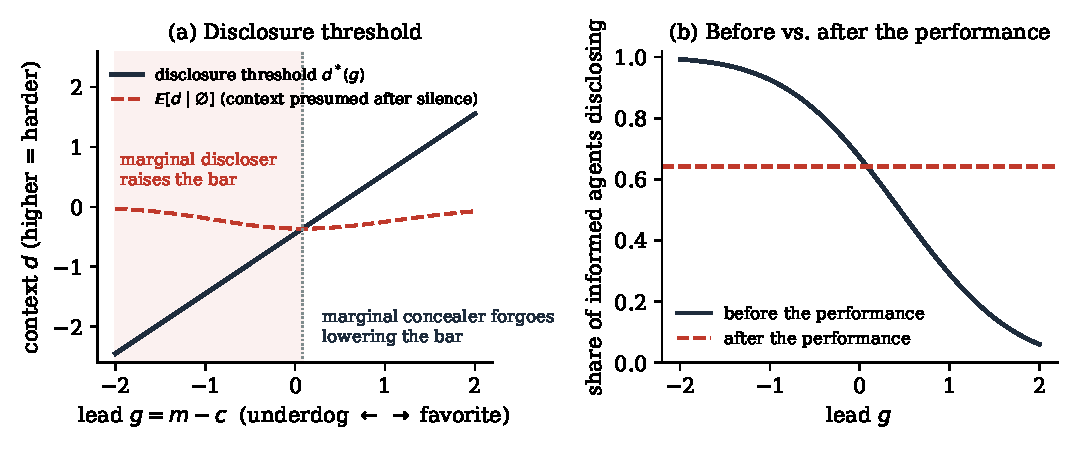
\includegraphics[width=\textwidth]{figures/fig_threshold.pdf}
\caption{Disclosure before a performance. Parameters: $q=0.6$, $\sth=\se=\sd=1$. (a) The threshold $d^*(g)$ from Theorem~\ref{thm:main} and the context the evaluator presumes after silence, $\E[d\mid\sil]$. To the left of $g_0$ the marginal discloser reveals a context easier than presumed (she raises the bar); to the right the marginal concealer hides a context harder than presumed (she forgoes lowering it). (b) The share of informed agents who disclose before the performance (Corollary~\ref{cor:standing}) and after it (Proposition~\ref{prop:timing}).}
\label{fig:threshold}
\end{figure}

\paragraph{What does the work.}
\begin{itemize}
\item \emph{Mechanism-essential.} Three ingredients are essential.
  \begin{itemize}
  \item The evaluator learns about talent from a performance that also reflects context, and reads worse performances as evidence of harder contexts (the monotone likelihood ratio of the Gaussian likelihood). This is the source of attribution.
  \item Hiring is a threshold decision. Without it standing is irrelevant (Proposition~\ref{prop:benchmarks}(c)).
  \item Disclosure precedes the performance. After it, standing is again irrelevant (Proposition~\ref{prop:timing}).
  \end{itemize}
\item \emph{Economically substantive.}
  \begin{itemize}
  \item Evidence is verifiable. Otherwise talk is cheap, by Proposition~\ref{prop:benchmarks}(b).
  \item Some agents lack evidence ($q<1$). As $q\to1$, $\beta(q)\to-\infty$ and unraveling is complete whatever the lead: the evaluator's attribution shifts the threshold but cannot stop unraveling on its own.
  \item Disclosure does not change the distribution of performance. This makes private information about talent irrelevant (Proposition~\ref{prop:private}), and it is what separates disclosing the benchmark from choosing a more or less benchmarkable project as in \citet{Zwiebel1995}.
  \end{itemize}
\item \emph{Tractability.} Normality of talent, noise and context delivers the closed form. Lemma~\ref{lem:pivotal} does not need it, and Section~\ref{sec:discussion} reports that the comparative static survives smooth payoffs.
\end{itemize}

\begin{corollary}[The evaluator learns least about favorites]\label{cor:learning}
The evaluator's expected residual uncertainty about talent, $\E\big[\Var(\theta\mid\mu,y)\big]$, is strictly increasing in the lead $g$.
\end{corollary}

Raising $g$ raises the threshold, so the information the evaluator receives at a higher lead is a garbling of the information at a lower lead. Favorites' performances are read against noisier benchmarks, so their reputations are tested less. In a repeated version this would make reputations sticky at the top. Figure~\ref{fig:regimes}(b) quantifies the effect.

%======================================================================
\section{``Preliminary'' versus ``polished''}\label{sec:noise}
%======================================================================

The difficulty of a context shifts the level of performance. Many disclaimers are instead about \emph{precision}: ``these results may change'', ``this is a first pass'', ``the sample is small''. To isolate this dimension, let performance be $y=\theta+\varepsilon_i$, where $\varepsilon_i\sim N(0,\sigma_i^2)$ and the agent's context is her noise type $i\in\{L,H\}$ with $\sigma_L<\sigma_H$. The prior probability of $L$ is $\pi\in(0,1)$. An informed agent (probability $q\in(0,1)$) holds verifiable evidence of $i$, and everything else is as before. Write $k_i:=\sth^2/(\sth^2+\sigma_i^2)$, so that $A(y,i)=m+k_i z$ with $k_L>k_H$.

\begin{proposition}[Preliminary versus polished]\label{prop:noise}
The equilibrium is unique, and no regularity assumption is needed. If $g>0$, informed agents disclose if and only if their performance is noisy ($i=H$): favorites say ``this is preliminary''. If $g<0$, informed agents disclose if and only if their performance is precise ($i=L$): underdogs say ``this is polished''.
\end{proposition}

After silence the evaluator weights performance by $\kappa(z):=\E[k_i\mid z,\sil]$, which lies strictly between $k_H$ and $k_L$ because the uninformed of both types are always silent. A favorite is hired unless $z$ is sufficiently negative, and on negative performances a lower weight is kinder, so the noisy type gains from disclosure and the precise type from silence. An underdog is hired only after sufficiently positive performances, where a higher weight is kinder. The argument is a pointwise comparison of hiring sets and does not use the pivotal lemma, which is why no monotonicity assumption is needed.

Taken together with Theorem~\ref{thm:main}, the model predicts \emph{what kind} of expectation management each side engages in. Favorites lower expectations only in the sense of lowering how much the performance counts: they say ``preliminary'', never ``hard''. Underdogs pin expectations down: they say ``hard'' when it is, ``polished'' when it is, and even disclose that their circumstances were favorable. This matches a familiar pattern: senior speakers call their work preliminary, while job-market candidates present polished work and explain how hard the data were to get. In the model the pattern comes from standing alone, without any signaling of talent.

%======================================================================
\section{Before or after: expectations versus excuses}\label{sec:timing}
%======================================================================

Suppose instead that the informed agent decides whether to disclose \emph{after} observing her performance. Give her any payoff that is strictly increasing in the assessment. The hiring indicator with a lexicographic preference for higher assessments is a special case.

\begin{proposition}[Excuses after the fact]\label{prop:timing}
With ex post disclosure, the unique equilibrium has informed agents disclose at performance $z$ if and only if $d>t(z):=-\rho z+\beta(q)\tau$. The rule does not depend on the lead $g$ or on the shape of the payoff. Consequently the probability that an informed agent discloses ex post is a constant $P_{\mathrm{post}}\in(0,1)$. Under Assumption~\ref{ass:R}, the ex ante probability $1-\Phi(d^*(g)/\sd)$ exceeds $P_{\mathrm{post}}$ for all sufficiently low $g$ and falls short of it for all sufficiently high $g$, crossing once.
\end{proposition}

Once the performance is known, disclosure is no longer a bet on how the performance will be read. The agent simply compares two assessments of a known performance and discloses whenever the truth beats the evaluator's inference. Ex post, the evaluator's inference and the agent's incentive depend on the realized performance but not on where the bar is. The contrast yields a sharp prediction: \emph{standing should predict what people say before a performance but not what they say after it.} In the example of Figure~\ref{fig:threshold}(b), $P_{\mathrm{post}}=0.64$, and ex ante disclosure falls from $0.93$ at $g=-1$ to $0.29$ at $g=1$.

%======================================================================
\section{Who wants context on the record?}\label{sec:mandates}
%======================================================================

Consider two institutional benchmarks. Under \emph{mandatory disclosure}, informed agents must disclose (think of course medians printed on transcripts, contextual admissions, or risk-adjusted surgical report cards). Under \emph{no disclosure}, context is never revealed.

\begin{proposition}[Transparency mandates]\label{prop:mandates}
The hiring probabilities are
\[
P_M=q\,\Phi\!\Big(\tfrac{g\sqrt V}{\sth^2}\Big)+(1-q)\,\Phi\!\Big(\tfrac{g\sqrt{V+\sd^2}}{\sth^2}\Big),
\qquad
P_B=\Phi\!\Big(\tfrac{g\sqrt{V+\sd^2}}{\sth^2}\Big),
\]
so $P_M>P_B$ if and only if $g<0$. The evaluator's expected payoff is weakly higher under mandatory disclosure than under both no disclosure and voluntary disclosure.
\end{proposition}

Underdogs gain from putting context on the record and favorites lose. Voluntary disclosure falls in between in our example (Figure~\ref{fig:regimes}(a)). The exception is a neighborhood of $g=0$, where voluntary disclosure is worst for the agent. There, adverse selection into silence penalizes uninformed agents, as in \citet{Dye1985}. The proposition gives a political-economy prediction: support for context mandates should come from those who are behind. It also offers a new reading of an old experience. When Cornell began printing course medians on transcripts, students shifted toward leniently graded courses \citep{BarKadiyaliZussman2009}. Our model adds that such mandates also redistribute across students by standing, independently of any course-choice response.

\begin{figure}[t]
\centering
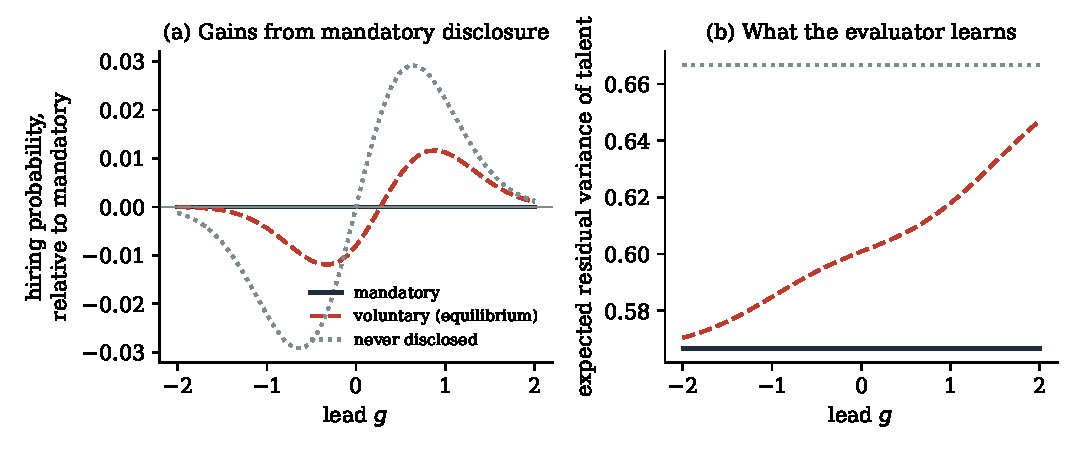
\includegraphics[width=\textwidth]{figures/fig_regimes.pdf}
\caption{Institutional regimes (same parameters as Figure~\ref{fig:threshold}). (a) Hiring probability under voluntary disclosure and no disclosure, relative to mandatory disclosure. (b) The evaluator's expected residual variance of talent; under voluntary disclosure it rises with the lead (Corollary~\ref{cor:learning}).}
\label{fig:regimes}
\end{figure}

%======================================================================
\section{Robustness and extensions}\label{sec:discussion}
%======================================================================

\paragraph{Smooth payoffs.} The hiring threshold is the cleanest way for standing to matter, but not the only one. Suppose the agent's payoff is $\Phi\big((A-c)/\omega\big)$: stakes that are S-shaped around the bar, which become the hiring indicator as $\omega\to0$ and linear as $\omega\to\infty$.

\begin{observation}\label{obs:smooth}
In the cases we computed ($\sth=\se=\sd=1$; $q=0.7$ with $\omega\in\{0.05,0.3,1,3,30\}$, and $q=0.6$ with $\omega\in\{0.3,1,3\}$), the equilibrium disclosure threshold is increasing in $g$ for every $\omega$. The slope decreases in $\omega$, from $\sd^2/\sth^2$ as $\omega\to0$ to $0$ as $\omega\to\infty$ (Figure~\ref{fig:smooth}).
\end{observation}

\begin{conjecture}
If the agent's payoff is $W(A-c)$ with $W$ increasing, convex on $(-\infty,0)$ and concave on $(0,\infty)$, the disclosure threshold is nondecreasing in $g$.
\end{conjecture}

The heuristic behind the conjecture is Lemma~\ref{lem:pivotal} ``smoothed''. With a general payoff, the agent compares assessments across all performances, weighting each by her marginal payoff. A favorite's weights concentrate on disappointments, where the evaluator's attribution is generous; an underdog's weights concentrate on surprises.

\begin{figure}[t]
\centering
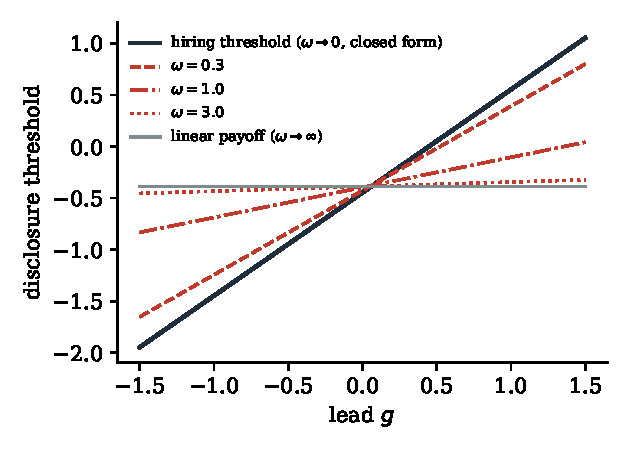
\includegraphics[width=0.55\textwidth]{figures/fig_smooth.pdf}
\caption{Disclosure threshold with payoff $\Phi\big((A-c)/\omega\big)$ (same parameters as Figure~\ref{fig:threshold}). The closed form of Theorem~\ref{thm:main} is the limit $\omega\to0$; linear payoffs ($\omega\to\infty$) make the threshold independent of standing.}
\label{fig:smooth}
\end{figure}

\paragraph{Regularity.} Assumption~\ref{ass:R} is used only to make the silent assessment increasing in performance for \emph{every} concealment set. For a threshold concealment set, the evaluator's posterior over contexts is a normal reweighted at a single point, whose variance is at most $\bar r(q)\,\tau^2$. Here $\bar r(q):=\sup_b\Var(X)$ in the notation of Appendix~\ref{app:proofs}, with $\bar r(0.5)\approx1.18$, $\bar r(0.6)\approx1.24$ and $\bar r(0.9)\approx1.68$. Under the weaker condition $\sd^2(\bar r(q)-1)<V$, the threshold \eqref{eq:dstar} is therefore still an equilibrium, and it is the unique equilibrium in which the silent assessment is monotone. When even this fails (very dispersed contexts, many informed concealers), the silent pool can be bimodal. A middling performance can then be read as a bad performance under easy circumstances, and the pivotal lemma no longer applies as stated.

\paragraph{Private information about talent.} One might expect an agent who knows something about her own talent to use disclosure to signal it, which would bring in the forces of \citet{Zwiebel1995}, \citet{FeltovichHarbaughTo2002} and \citet{HarbaughTo2020}. With a hiring threshold she does not.

\begin{proposition}[Private information about talent]\label{prop:private}
Suppose the informed agent also privately observes a signal $s$ of her talent, where $(\theta,s)$ is independent of $(d,\varepsilon)$ and of whether the agent is informed, and $y$ has full support given $(d,s)$. Then the strategies and beliefs of Theorem~\ref{thm:main}, in which disclosure depends on $d$ alone, remain an equilibrium. Moreover, in any equilibrium in which assessments are increasing in performance, two informed agents with the same context who strictly prefer a message prefer the same one, whatever their signals. The same holds for Propositions~\ref{prop:noise} and~\ref{prop:timing}.
\end{proposition}

The reason is Lemma~\ref{lem:pivotal} once more. The agent's message selects a bar but leaves the distribution of her performance unchanged. Knowing more about her talent changes that distribution, but not the ranking of bars: a lower bar is better for everyone. Because disclosure decisions do not depend on the signal, silence and disclosure carry no information about talent beyond what the context itself carries. This is the sharpest difference from project choice in \citet{Zwiebel1995}, where the chosen project changes the performance technology and different types therefore rank projects differently. With smooth payoffs the irrelevance result fails, since the agent's signal then determines which performances carry weight in her payoff. Attribution and signaling would then interact; we leave this to future work.

\paragraph{Commitment.} If an institution (or the agent, before learning her context) can commit to a disclosure policy about context, the problem becomes Bayesian persuasion in which the instrument is information about a nuisance parameter and the payoff-relevant information arrives exogenously afterwards (compare \citealp{BizzottoRudigerVigier2021}). Within linear-Gaussian policies the answer is the extreme one of Proposition~\ref{prop:mandates}: no information for favorites, full information for underdogs. The optimal nonlinear policy (for example, revealing only extreme contexts) is open.

\paragraph{Dynamics.} Corollary~\ref{cor:learning} suggests a mechanism for persistent reputations. Agents who are ahead keep their performances hard to read, which slows learning about them. A dynamic version would ask whether this produces a Matthew effect in reputations.

\paragraph{Non-Bayesian audiences.} If the audience adopts whatever narrative about circumstances best fits the data \citep{SchwartzsteinSunderam2021} or reasons with competing causal narratives \citep{EliazSpiegler2020}, cheap talk about context can matter. Our results are the Bayesian benchmark against which such narrative effects can be measured.

%======================================================================
\section{Related literature}\label{sec:lit}
%======================================================================

\paragraph{Verifiable disclosure.} The unraveling result of \citet{Grossman1981} and \citet{Milgrom1981} fails when the receiver is unsure whether the sender has evidence \citep{Dye1985,JungKwon1988,Shin1994}. Our equilibrium inherits the Dye structure: equation \eqref{eq:beta} is the Dye constant. The object disclosed, however, is different. In the standard model the disclosed variable is the receiver's object of interest. Here it is payoff-irrelevant to the evaluator, and it matters only for how he reads a performance that neither party controls. This is why standing matters, and why it matters through the pivotal performance.

\citet{BenPorathDekelLipman2018} study how the prospect of disclosure shapes project choice, and \citet{HartKremerPerry2017} study commitment in evidence games. The closest disclosure models are those in which the receiver also observes exogenous information:
\begin{itemize}
\item \citet{AcharyaDeMarzoKremer2011} on the timing of disclosure relative to market news;
\item \citet{FrenkelGuttmanKremer2020} on third-party information;
\item \citet{LibgoberMichaeliWiedman2023}, where silence is interpreted in light of external news of uncertain veracity.
\end{itemize}
In all of these the exogenous and disclosed information concern the same payoff-relevant value. In accounting, \citet{HughesPae2004} and \citet{KimPae2025} study the disclosure of the \emph{precision} of a value signal, which is related in spirit to Proposition~\ref{prop:noise}. Their payoffs are linear in prices, however, so standing plays no role, and their disclosure is ex post.

\paragraph{Career concerns and informativeness.} In career-concerns models \citep{Holmstrom1999,DewatripontJewittTirole1999}, the informativeness of performance is central. That agents ahead of a firing or promotion threshold prefer less informative evaluations is familiar from \citet{Hermalin1993} and, above all, \citet{Zwiebel1995}. There, managers who know their ability choose between an industry-standard project, which is evaluated against an accurate benchmark, and an innovation that is not; very high and very low ability managers innovate, while average ones conform.

Our paper differs in three ways:
\begin{itemize}
\item the instrument is disclosure of the benchmark rather than a choice of technology;
\item nothing is signaled, even when the agent has private information about her ability (Proposition~\ref{prop:private}), because disclosure changes how performance is read but not its distribution;
\item the main results (underdogs raising the bar, the difficulty versus noise dichotomy, and the timing contrast) have no counterpart there.
\end{itemize}
The idea that a Bayesian evaluator filters common shocks goes back to relative performance evaluation \citep{Holmstrom1982}.

\paragraph{Persuasion and information design.} The preference of favorites for less information and of underdogs for more is the concavification logic of \citet{KamenicaGentzkow2011}. Informed senders who choose the informativeness of a test are studied by \citet{PerezRichet2014}, \citet{Hedlund2017}, \citet{DeganLi2021} and \citet{KoesslerSkreta2023}, where the choice of experiment signals the sender's type. Our agent cannot commit, and the information she controls concerns the \emph{interpretation} of an exogenous signal rather than the state. \citet{BizzottoRudigerVigier2021} study persuasion alongside exogenous information arriving over time.

\paragraph{Countersignaling and modesty.} \citet{FeltovichHarbaughTo2002} show that high types may refrain from signaling when the receiver has other information. \citet{HarbaughTo2020} show that withholding good news (such as a title) can be an equilibrium when standards are easy or prior expectations favorable, because the weakest senders gain most from disclosure. The conclusion that favorites withhold favorable evidence is similar. The mechanism is not: in our model nothing is signaled, even when the agent knows her talent (Proposition~\ref{prop:private}), and concealment arises from attribution at the pivotal performance.

\paragraph{Reference points, expectations and emotions.} Kőszegi and Rabin's expectation-based reference points \citeyearpar{KoszegiRabin2006,KoszegiRabin2009} give a psychological reason why exceeding expectations feels good. Information design with belief-based utility includes suspense and surprise \citep{ElyFrankelKamenica2015}, news utility with diminishing sensitivity \citep{DurajHe2024}, disclosure to a psychological audience \citep{LipnowskiMathevet2018} and emotional agency \citep{Koszegi2006}. \citet{ZeckhauserViscusi2025} document and model people deliberately lowering their \emph{own} expectations; see also \citet{GollierMuermann2010} and \citet{BrunnermeierParker2005}. \citet{Robertson2025} studies persuasion of a judge whose reference point shifts the conviction threshold. Our contribution relative to this line is to show that judging relative to expectations, and managing those expectations, arises with standard preferences once the audience learns about a person from a performance.

\paragraph{Attribution, narratives and self-handicapping.} \citet{BenabouTirole2002} rationalize self-handicapping as self-signaling, and \citet{XiangGershmanGerstenberg2026} model it as signaling to observers, finding that it works on naive observers and backfires on sophisticated ones. Excuses made in advance are the verbal cousin of self-handicapping, and our Bayesian evaluator is maximally sophisticated. \citet{HeidhuesKoszegiStrack2018} study misattribution of performance by overconfident agents, and \citet{SchwartzsteinSunderam2021} and \citet{EliazSpiegler2020} study persuasion through models and narratives.

\paragraph{Applications.} In political economy, \citet{AshworthBdMFriedenberg2017} show that voters' information about circumstances shapes both accountability and selection. \citet{Garro2019} rationalizes why front-runners avoid debates, and \citet{CaseyGlennerster2024} document this empirically. In finance and accounting, the walk-down of forecasts \citep{Matsumoto2002,RichardsonTeohWysocki2004} and the joint determination of forecasts and earnings management \citep{Beyer2009} are the canonical expectation-management phenomena. \citet{Stein1989} supplies the signal-jamming logic by which anticipated manipulation can persist without fooling anyone. In education, the Cornell median-grade experiment \citep{BarKadiyaliZussman2009} and test-optional admissions \citep{DesseinFrankelKartik2025} are policies about what context an evaluator sees.

\begin{table}[t]
\centering
\small
\begin{tabularx}{\textwidth}{@{}>{\raggedright\arraybackslash}p{3.3cm}>{\raggedright\arraybackslash}X>{\raggedright\arraybackslash}X@{}}
\toprule
Paper & What is shared & What differs here \\
\midrule
\citet{Zwiebel1995} & Value of an accurate benchmark depends on position relative to a firing threshold & Instrument is disclosure of the benchmark, which leaves the performance technology unchanged, so nothing is signaled even with private ability information; underdogs raise the bar; difficulty versus noise; timing \\
\citet{HarbaughTo2020} & Favorable evidence withheld when priors are favorable & No signaling of type; disclosed variable is payoff-irrelevant context; mechanism is attribution at the pivot \\
\citet{Dye1985}; \citet{JungKwon1988} & Uncertain evidence endowment, threshold equilibrium, same constant $\beta(q)$ & Standing matters here but not in the standard model (Prop.~\ref{prop:benchmarks}(c)); disclosure interacts with a later exogenous signal \\
\citet{KamenicaGentzkow2011}; \citet{Hermalin1993} & Favorites prefer less informative evaluations & No commitment; which contexts are disclosed is pinned down by attribution, not by informativeness alone \\
\citet{HughesPae2004}; \citet{KimPae2025} & Disclosure of precision of a signal & Career-threshold payoffs; ex ante vs.\ ex post; difficulty (location) as well as noise \\
\citet{LibgoberMichaeliWiedman2023}; \citet{FrenkelGuttmanKremer2020} & Silence read in light of other information & There, disclosed and outside information concern the same value; here the outside signal concerns talent and the disclosed variable is a nuisance parameter \\
\bottomrule
\end{tabularx}
\caption{Closest papers.}
\label{tab:lit}
\end{table}

%======================================================================
\section{Conclusion}
%======================================================================

The folk rule says to lower expectations and then exceed them. With a Bayesian audience expectations cannot be lowered on average, and talk about circumstances is ignored unless it is verifiable. Once verifiable, it changes how the audience attributes performance to talent. The evaluator's own attribution excuses disappointments and discounts surprises. So favorites, who are judged on their disappointments, leave the excusing to the evaluator and at most say that the performance is preliminary. Underdogs, who are judged on their surprises, pin the context down and even raise the bar. The same people who stay quiet before a performance may make excuses after it, because after the fact standing no longer matters.

Three questions seem most promising next: smooth stakes combined with private information about talent, where attribution and signaling interact; optimal (committed) context disclosure by institutions; and the dynamics of reputations when those ahead keep their performances hard to read.

\bibliographystyle{plainnat}
\bibliography{references}

\appendix
%======================================================================
\section{Proofs}\label{app:proofs}
%======================================================================

\paragraph{A reweighted normal.} For $b\in\R$ and $q\in(0,1)$ let $X$ have density proportional to $\phi(x)w_b(x)$ with $w_b(x)=\mathbf 1\{x<b\}+(1-q)\mathbf 1\{x\ge b\}$. Direct integration gives
\[
\E[X]=-h(b),\qquad \E[X^2]=1-b\,h(b),\qquad h(b):=\frac{q\,\phi(b)}{1-q+q\Phi(b)} ,
\]
so $\Var(X)=1-b\,h(b)-h(b)^2$. Let $f(b):=b+h(b)$. Since $h'(b)=-b\,h(b)-h(b)^2$, we have $f'(b)=\Var(X)>0$. Moreover $f(b)\to-\infty$ as $b\to-\infty$ and $f(b)\to\infty$ as $b\to\infty$ (because $h\to0$ in both limits when $q<1$), and $f(0)>0$. Hence $f$ has a unique root $\beta(q)<0$, which is \eqref{eq:beta}. If $Y$ has density proportional to $\phi\big((y-a)/\tau\big)\big[\mathbf 1\{y<t\}+(1-q)\mathbf 1\{y\ge t\}\big]$, then $Y=a+\tau X$ with $b=(t-a)/\tau$, so $\E[Y]=a-\tau h\big((t-a)/\tau\big)$.

\paragraph{Proof of Lemma~\ref{lem:monotone}.} By \eqref{eq:As}, $\partial A(y,\sil)/\partial y=k\,\big(1-\Var(d\mid z,\sil)/V\big)$. To see this, differentiate the posterior $p(d\mid z)\propto h_N(d)\exp\{-(z+d)^2/(2V)\}$, which gives $\partial_z\E[d\mid z]=-\Var(d\mid z)/V$. The posterior is a $N(-\rho z,\tau^2)$ density reweighted by $w(d)\in[1-q,1]$, so
\[
\Var(d\mid z,\sil)\le \frac{\int (d+\rho z)^2 w(d)\,\phi\big(\tfrac{d+\rho z}{\tau}\big)\,dd}{\int w(d)\,\phi\big(\tfrac{d+\rho z}{\tau}\big)\,dd}\le\frac{\tau^2}{1-q}.
\]
Assumption~\ref{ass:R} is equivalent to $\tau^2/(1-q)<V$. So the slope is bounded below by $k\big(1-\tau^2/((1-q)V)\big)>0$, which gives monotonicity and unboundedness. Continuity is immediate. \hfill$\square$

\paragraph{Proof of Lemma~\ref{lem:pivotal}.} The distribution of $y$ given $\omega$ does not depend on the message and has full support. Under message $x\in\{\omega,\sil\}$ the agent is hired if and only if $y\ge\bar y_x$, where $\bar y_x$ is the unique solution of $A(\bar y_x,x)=c$. So she strictly prefers disclosure if and only if $\bar y_\omega<\bar y_\sil$. Since $A(\cdot,\omega)$ is strictly increasing, this holds if and only if $A(\bar y_\sil,\omega)>A(\bar y_\omega,\omega)=c$. The reverse inequality works the same way. In the Gaussian model, \eqref{eq:Ad} and \eqref{eq:As} give $A(\bar y_\sil,d)-c=A(\bar y_\sil,d)-A(\bar y_\sil,\sil)=k\,\big(d-\E[d\mid\bar z_\sil,\sil]\big)$. \hfill$\square$

\paragraph{Proof of Proposition~\ref{prop:benchmarks}.}
\begin{enumerate}[label=(\alph*)]
\item Both statements are the law of iterated expectations.
\item Under the stated monotonicity, each on-path message $\mu$ induces a bar $\bar y_\mu$. The hiring probability of any type, $\Pr(y\ge\bar y_\mu\mid\text{type})$, is strictly decreasing in $\bar y_\mu$ because $y$ has full support. Hence every type sends a message with the lowest on-path bar, so all on-path messages share a bar $\bar y$ and $A(\bar y,\mu)=c$ for all of them. The assessment without communication is $\E[\theta\mid y]=\sum_\mu\Pr(\mu\mid y)A(y,\mu)$, which equals $c$ at $\bar y$. By monotonicity, $\bar y$ is the bar without communication, so each type is hired exactly when she would be without communication.
\item With payoff $\alpha+\gamma A$ ($\gamma>0$), an informed agent compares $\E[A(y,d)\mid d]$ with $\E[A(y,\sil)\mid d]$. By \eqref{eq:Ad}--\eqref{eq:As}, both equal $m$ plus $k$ times an expectation over $z\sim N(-d,V)$ that involves only $d$ and the silent pool. So the best-response correspondence, and hence the equilibrium set, is independent of $(m,c)$. \hfill$\square$
\end{enumerate}

\paragraph{Proof of Theorem~\ref{thm:main}.} Take any equilibrium with concealment set $N$. By Lemma~\ref{lem:monotone} the silent assessment is strictly increasing and unbounded, so the silent bar $\bar z_\sil$ exists and is unique. By Lemma~\ref{lem:pivotal} an informed agent discloses if $d>t$ and conceals if $d<t$, where $t:=\E[d\mid\bar z_\sil,\sil]$. Hence $N=(-\infty,t)$ up to a null set.

Next, $A(\bar y_\sil,\sil)=c$ and \eqref{eq:As} give $\bar z_\sil+t=-g/k=-gV/\sth^2$. At $(\bar z_\sil,\sil)$ the posterior density of $d$ is proportional to
\[
\phi(d/\sd)\,\phi\big((\bar z_\sil+d)/\sqrt V\big)\,w_t(d)\;\propto\;\phi\big((d-a)/\tau\big)\,w_t(d),\qquad a:=-\rho\,\bar z_\sil=\rho\,\big(t+gV/\sth^2\big),
\]
with $w_t(d)=\mathbf 1\{d<t\}+(1-q)\mathbf 1\{d\ge t\}$. By the reweighted-normal formula, $t=a-\tau h\big((t-a)/\tau\big)$, that is, $f\big((t-a)/\tau\big)=0$. So $(t-a)/\tau=\beta(q)$. Substituting $a$ gives $t(1-\rho)=\rho gV/\sth^2+\beta\tau$. Using $\rho/(1-\rho)=\sd^2/V$ and $\tau/(1-\rho)=\sd\sqrt{(\sd^2+V)/V}$ yields \eqref{eq:dstar}.

For existence, let $t=d^*(g)$ and define $\bar z:=-t-gV/\sth^2$. The computation above shows $\E[d\mid\bar z,\sil]=t$, so $A(\bar y,\sil)=m+k(\bar z+t)=c$, and $\bar z$ is the silent bar. By Lemma~\ref{lem:pivotal} the threshold rule is a best response, beliefs follow Bayes' rule after silence, and disclosure is verifiable. So this is an equilibrium, and by the first part it is the only one. \hfill$\square$

\paragraph{Proof of Corollary~\ref{cor:standing}.} This follows immediately from \eqref{eq:dstar}. \hfill$\square$

\paragraph{Proof of Corollary~\ref{cor:raise}.} The silent pool before the performance is $N(0,\sd^2)$ reweighted by $w_{d^*}$, so $\E[d\mid\sil]=-\sd\,h(d^*/\sd)$. Hence $d^*<\E[d\mid\sil]$ if and only if $f(d^*/\sd)<0$, if and only if $d^*<\beta\sd$ (since $f$ is increasing with root $\beta$). By \eqref{eq:dstar} this is equivalent to $g\,\sd^2/\sth^2<\beta\sd\big(1-\sqrt{1+\sd^2/V}\big)$, that is, $g<g_0$. Since $\beta<0$ and $1-\sqrt{1+\sd^2/V}<0$, we have $g_0>0$. \hfill$\square$

\paragraph{Proof of Corollary~\ref{cor:learning}.} Let $g'>g$, so $d^*(g')>d^*(g)$. The message under $g'$ is a function of the message under $g$: it equals the disclosed $d$ if $d\ge d^*(g')$ and $\sil$ otherwise. Hence $\sigma(\mu_{g'},y)\subseteq\sigma(\mu_g,y)$, and $\E[\Var(\theta\mid\mu_{g'},y)]\ge\E[\Var(\theta\mid\mu_g,y)]$. The inequality is strict because on the event $\{\text{informed},\,d\in[d^*(g),d^*(g'))\}$, which has positive probability, $\E[\theta\mid\mu_{g},y]=m+k(z+d)$ differs from $\E[\theta\mid\mu_{g'},y]$ on a set of positive probability. \hfill$\square$

\paragraph{Proof of Proposition~\ref{prop:noise}.} For any strategy of the informed, the silent pool contains uninformed agents of both types with positive weight. So $\kappa(z):=\E[k_i\mid z,\sil]\in(k_H,k_L)$ for every $z$, and $A(y,\sil)=m+\kappa(z)z$. Type $i$ is hired after disclosure if and only if $k_iz\ge -g$, and after silence if and only if $\kappa(z)z\ge -g$.

\emph{Case $g>0$.} Every $z\ge0$ leads to hiring under both messages. For $z<0$, $k_Hz>\kappa(z)z>k_Lz$. Hence the disclosure hiring set of type $H$ strictly contains the silent hiring set, which strictly contains the disclosure hiring set of type $L$. Each containment differs by a set of positive Lebesgue measure, by continuity of $\kappa$ and the strict inequalities near the boundary $z=-g/k_i$. Since $z$ has full support, $H$ strictly prefers disclosure and $L$ strictly prefers silence.

\emph{Case $g<0$.} No $z\le0$ leads to hiring. For $z>0$, $k_Lz>\kappa(z)z>k_Hz$, and the same argument applies with the roles reversed.

Best responses do not depend on the pool beyond $\kappa\in(k_H,k_L)$, so the equilibrium is unique. \hfill$\square$

\paragraph{Proof of Proposition~\ref{prop:timing}.} After observing $z$, the agent's payoff is strictly increasing in her assessment (or lexicographically so). She therefore discloses if $A(y,d)>A(y,\sil)$, that is, if $d>\E[d\mid z,\sil]$. Here the silent pool at $z$ consists of uninformed agents and informed agents with $d<t(z)$. Given $z$, the prior of $d$ updated by the performance is $N(-\rho z,\tau^2)$. The equilibrium condition $t(z)=\E[d\mid z,\sil]$ is therefore the reweighted-normal fixed point with $a=-\rho z$, which gives $t(z)=-\rho z+\beta\tau$, unique for each $z$. This rule involves neither $g$ nor the payoff. The ex post disclosure probability is $P_{\mathrm{post}}=\E_d\big[\Pr(d>-\rho Z+\beta\tau)\big]$ with $Z\sim N(-d,V)$, which lies strictly in $(0,1)$. The ex ante probability $1-\Phi(d^*(g)/\sd)$ is continuous, strictly decreasing, and has limits $1$ and $0$ (Corollary~\ref{cor:standing}), so it crosses $P_{\mathrm{post}}$ exactly once. \hfill$\square$

\paragraph{Proof of Proposition~\ref{prop:mandates}.} After disclosure $A=m+k(z+d)$ with $z+d\sim N(0,V)$, so the hiring probability is $\Phi(g/(k\sqrt V))=\Phi(g\sqrt V/\sth^2)$. Without disclosure, $z\sim N(0,V+\sd^2)$ and $A=m+k_0z$ with $k_0=\sth^2/(V+\sd^2)$, so the hiring probability is $\Phi(g\sqrt{V+\sd^2}/\sth^2)$. Under the mandate, silence reveals that the agent is uninformed, which gives $P_M$. Since $\sqrt{V+\sd^2}>\sqrt V$, $P_M>P_B$ if and only if $g<0$. The evaluator's information under the mandate is Blackwell more informative than under either alternative, because both alternatives' messages are functions of the mandated message and $y$. \hfill$\square$

\paragraph{Proof of Proposition~\ref{prop:private}.} Fix the evaluator's beliefs of Theorem~\ref{thm:main}. After either message $x\in\{d,\sil\}$ the evaluator hires if and only if $y\ge\bar y_x$, with the bars of Theorem~\ref{thm:main}. An informed agent with $(d,s)$ is hired with probability $\Pr(y\ge\bar y_x\mid d,s)$, which is strictly decreasing in $\bar y_x$ by full support. So she discloses if and only if $\bar y_d<\bar y_\sil$, that is, if and only if $d>d^*(g)$, whatever her signal $s$. Disclosure then depends only on $d$, and $(\theta,s)$ is independent of $d$ and of being informed. So the evaluator's beliefs about $\theta$ after $(y,\mu)$ coincide with those of Theorem~\ref{thm:main}, which proves the first claim.

For the second claim, take any equilibrium with increasing assessments. The hiring set after each message is an upper set $\{y\ge\bar y_x\}$. An informed agent with context $d$ chooses between the bars $\bar y_d$ and $\bar y_\sil$, which depend on $d$ but not on $s$. If $\bar y_d\ne\bar y_\sil$, all agents with context $d$ strictly prefer the lower bar.

The same reasoning covers the other two results. The proof of Proposition~\ref{prop:noise} compares hiring sets pointwise and does not involve the distribution of performance. In Proposition~\ref{prop:timing} the agent compares two assessments at a known performance, which do not depend on $s$. \hfill$\square$


%======================================================================
\section{Numerical details}\label{app:numerics}
%======================================================================

All figures are produced by \texttt{code/figures.py}, using the module \texttt{code/model.py}. Posteriors over the context are computed on a grid of $4{,}001$ points on $[-9\sd,9\sd]$ in log space. The closed form \eqref{eq:dstar} was checked against a brute-force fixed point, solving for the silent bar and the pivotal inference by root-finding, for $(q,\sd,\sth^2,\se^2)$ equal to $(0.5,1,1,1)$, $(0.6,1,1,1)$, $(0.7,1,1,1)$, $(0.9,1,1,1)$, $(0.7,2,1,1)$, $(0.7,0.5,1,0.5)$ and $(0.7,1,2,0.5)$, and $g\in\{-1,0,1\}$. It agrees to four decimals in every case, including cases that satisfy only the weaker regularity condition discussed in Section~\ref{sec:discussion}. The smooth-payoff thresholds in Figure~\ref{fig:smooth} solve the indifference condition of the marginal type by quadrature over performance, with $121$ nodes.

\end{document}
